\documentclass[draft]{article}

% PACKAGES
\usepackage[utf8]{inputenc}
\usepackage{amsmath,amssymb,mathtools}
\usepackage{ntheorem}
\usepackage[margin=4cm]{geometry}
\usepackage[final]{listings}
\usepackage{xcolor, color}
\usepackage{algorithm} % for algorithm environment
\usepackage[final]{graphicx}
\usepackage{setspace}
\usepackage{float}
\usepackage{multirow, multicol}
\usepackage{enumitem}
\usepackage{ifdraft}
\usepackage{xspace}
\usepackage{enumitem}
\usepackage{tabularx,comment}
\usepackage{soul}
\usepackage{scalefnt} % scale font
\usepackage{mdframed} % frame figures
\usepackage{pifont} % tick and cross
\usepackage{parskip} % no indentation and paragraph spacing
\usepackage[pdfpagelabels=true,backref=page,bookmarks=true]{hyperref} % KEEP AT THE END OF THE IMPORTS

\ifdraft{\usepackage[colorinlistoftodos, textwidth = 30mm]{todonotes}}{\usepackage[disable, colorinlistoftodos, textwidth = 30mm]{todonotes}}

% Colors
\definecolor{cred}{rgb}{1, 0.5, 0.5}
\definecolor{cgreen}{rgb}{0.5, 1, 0.5}
\definecolor{cblue}{rgb}{0.5, 0.5, 1}

% Hyperref setup
\hypersetup{
    final=true,
    colorlinks=true,
    linkcolor=cblue,
    urlcolor=cred,
    citecolor=teal,
}

% Draft mode changes:  
% https://tex.stackexchange.com/questions/49277/what-does-the-draft-mode-change
% ===== SETTINGS =====
\pagestyle{plain}

% Margins
\textwidth 18 cm
\textheight 22 cm
\topmargin -1 cm
\oddsidemargin -1 cm

% Directories
\newcommand{\definedir}[2]{\newcommand{#1}{#2}}
\definedir{\secs}{../secs}
\definedir{\figs}{../images}

% Style
\definecolor{codegreen}{rgb}{0,0.6,0}
\definecolor{codegray}{rgb}{0.5,0.5,0.5}
\definecolor{codepurple}{rgb}{0.58,0,0.82}
\definecolor{backcolour}{rgb}{0.95,0.95,0.92}
\lstdefinestyle{mystyle}{
    backgroundcolor=\color{backcolour},   
    commentstyle=\color{codegreen},
    keywordstyle=\color{magenta},
    numberstyle=\tiny\color{codegray},
    stringstyle=\color{codepurple},
    basicstyle=\ttfamily\normalsize,
    breakatwhitespace=false,         
    breaklines=true,                 
    captionpos=b,                    
    keepspaces=true,                 
    numbers=left,                    
    numbersep=5pt,                  
    showspaces=false,                
    showstringspaces=false,
    showtabs=false,                  
    tabsize=2
}
\lstset{style=mystyle}

% Footnote style
\let\svthefootnote\thefootnote
\newcommand\freefootnote[1]{%
  \let\thefootnote\relax%
  \footnotetext{#1}%
  \let\thefootnote\svthefootnote%
}

\setlength{\skip\footins}{2pc}

%Enumerate (1 -> 1.1 -> 1.1.1)
\renewcommand{\labelenumii}{\theenumii}
\renewcommand{\theenumii}{\theenumi.\arabic{enumii}.}

% ===== MACROS =====

% Comments
\newcommand{\todotag}{\sethlcolor{red}\hl{ to-do }\xspace}
\newcommand{\js}[1]{{\todo[size=\small, color=blue!40]{Javier: #1}}}
\newcommand{\jsi}[1]{{\todo[inline, size=\small, color=blue!40]{Javier: #1}}}
\newcommand{\mb}[1]{{\todo[size=\small, color=red!40]{Marta: #1}}}
\newcommand{\mbi}[1]{{\todo[inline, size=\small, color=red!40]{Marta: #1}}}
\newcommand{\dk}[1]{{\todo[size=\small, color=orange!40]{Dmitry: #1}}}
\newcommand{\dki}[1]{{\todo[inline, size=\small, color=orange!40]{Dmitry: #1}}}
\newcommand{\zp}[1]{{\todo[size=\small, color=red!40]{Zaira: #1}}}
\newcommand{\zpi}[1]{{\todo[inline, size=\small, color=green!40]{Zaira: #1}}}
\newcommand{\xs}[1]{{\todo[size=\small, color=red!40]{Xavier: #1}}}
\newcommand{\xsi}[1]{{\todo[inline, size=\small, color=purple!40]{Xavier: #1}}}

% Hyperlinks
\newcommand{\hlset}[1]{\hypertarget{\detokenize{#1}}{#1}}
\newcommand{\hlget}[1]{\hyperlink{\detokenize{#1}}{#1}}

% Mathbb
\newcommand{\N}{\mathbb{N}}
\newcommand{\Z}{\mathbb{Z}}
\newcommand{\E}{\mathbb{E}}
\newcommand{\F}{\mathbb{F}}
\newcommand{\G}{\mathbb{G}}
\newcommand{\Q}{\mathbb{Q}}
\newcommand{\R}{\mathbb{R}}
\newcommand{\J}{\mathbb{J}}
\newcommand{\B}{\mathbb{B}}

% Mathsf
\newcommand{\klic}{\mathsf{k_{lic}}}
\newcommand{\kreq}{\mathsf{k_{req}}}
\newcommand{\kdh}{\mathsf{k_{DH}}}
\newcommand{\ksym}{\mathsf{k}}
\newcommand{\tkdh}{\mathsf{\tilde{k}_{DH}}}
\newcommand{\tklic}{\mathsf{\tilde{k}_{lic}}}
\newcommand{\tkreq}{\mathsf{\tilde{k}_{req}}}
\newcommand{\sk}{\mathsf{sk}}
\newcommand{\pk}{\mathsf{pk}}
\newcommand{\ck}{\mathsf{ck}}
\renewcommand{\pk}{\mathsf{pk}}
\newcommand{\vk}{\mathsf{vk}}
\newcommand{\npk}{\mathsf{npk}}
\newcommand{\user}{\mathsf{user}}
\newcommand{\NFT}{\mathsf{NFT}}
\newcommand{\LP}{\mathsf{LP}}
\newcommand{\SP}{\mathsf{SP}}
\newcommand{\npkn}[1]{\mathsf{npk}_{#1}}
\newcommand{\nsk}{\mathsf{nsk}}
\newcommand{\lsk}{\mathsf{lsk}}
\newcommand{\lpk}{\mathsf{lpk}}
\newcommand{\rpk}{\mathsf{rpk}}
\newcommand{\spk}{\mathsf{spk}}
\newcommand{\tx}{\mathsf{tx}}
\newcommand{\txold}{\mathsf{tx^{old}}}
\newcommand{\txm}{\mathsf{tx_{metadata}}}
\newcommand{\txp}{\mathsf{tx_{payload}}}
\newcommand{\txh}{\mathsf{tx_{hash}}}
\newcommand{\txproof}{\mathsf{tx_{proof}}}
\newcommand{\Note}{\mathsf{N}}
\newcommand{\lic}{\mathsf{lic}}
\newcommand{\req}{\mathsf{req}}
\newcommand{\Session}{\mathsf{session}}
\newcommand{\SessionCookie}{\mathsf{sc}}
\newcommand{\nfthash}{\mathsf{hash_{NFT}}}
\newcommand{\nftpayload}{\mathsf{payload_{NFT}}}
\newcommand{\sig}{\mathsf{sig}}
\newcommand{\lsig}{\mathsf{sig_{lic}}}
\newcommand{\tsig}{\mathsf{sig_{tx}}}
\newcommand{\attr}{\mathsf{attr}}
\newcommand{\attrdata}{\mathsf{attr\_data}}
\newcommand{\sign}{\mathsf{sign\_single\_key}}
\newcommand{\signd}{\mathsf{sign\_double\_key}}
\newcommand{\verify}{\mathsf{verify\_sig\_single\_key}}
\newcommand{\verifyd}{\mathsf{verify\_sig\_double\_key}}
\newcommand{\mintnft}{\mathsf{mint\_nft}}
\newcommand{\NoteB}{\mathsf{N_{B}}}
\newcommand{\NoteC}{\mathsf{N_{C}}}
\newcommand{\nnew}[1]{\mathsf{N^{new}_{#1}}}
\newcommand{\nold}[1]{\mathsf{N^{old}_{#1}}}
\newcommand{\vnew}[1]{\mathsf{v_{#1}}}
\newcommand{\vold}[1]{\mathsf{w_{#1}}}
\newcommand{\change}{\mathsf{change}}
\newcommand{\type}{\mathsf{type}}
\newcommand{\com}{\mathsf{com}}
\newcommand{\enc}{\mathsf{enc}}
\newcommand{\nonce}{\mathsf{nonce}}
\newcommand{\pos}{\mathsf{pos}}
\newcommand{\nullifier}{\mathsf{nullifier}}
\newcommand{\isseen}{\mathsf{is\_seen}}
\newcommand{\pnullifiers}{\mathsf{previous\_nullifiers}}
\newcommand{\sessionid}{\mathsf{session\_id}}
\newcommand{\hb}{H^\mathsf{BLAKE2b}}
\newcommand{\hp}{H^\mathsf{Poseidon}}

% Mathfrak
\newcommand{\Ftuple}{\mathfrak{F}}
\newcommand{\Bitstrings}{\mathfrak{B}}

% Misc maths
\newcommand{\floor}[1]{\lfloor #1 \rfloor}
\newcommand{\ceil}[1]{\lceil #1 \rceil}

% Misc cryptography
\newcommand{\sample}{\xleftarrow{\$}}
\newcommand{\error}{\perp}
\newcommand{\conc}{\;||\;}
\newcommand{\snull}{\sf{null}}

% Building blocks
\renewcommand{\SS}{\sf{S}}
\newcommand{\EE}{\sf{E}}
\newcommand{\CC}{\sf{C}}
\newcommand{\PP}{\sf{P}}
\newcommand{\MT}{\sf{MT}}
\newcommand{\NN}{\sf{N}}

% Cryptographic algorithms
\newcommand{\Setup}{\sf{Setup}}
\newcommand{\SetupU}{\sf{SetupUniversal}} % find a better one
\newcommand{\SetupD}{\sf{SetupDependent}} % find a better one
\newcommand{\Com}{\sf{Com}}
\newcommand{\Hash}{\sf{Hash}}
\newcommand{\Enc}{\sf{Enc}}
\newcommand{\Dec}{\sf{Dec}}
\newcommand{\SDec}{\sf{SymDec}}
\newcommand{\Sign}{\sf{Sign}}
\newcommand{\Prove}{\sf{Prove}}
\newcommand{\Verify}{\sf{Verify}}
\newcommand{\Nul}{\sf{Nullify}}
\newcommand{\Open}{\sf{Open}}
\newcommand{\UpdateCom}{\sf{UpdateCom}}
\newcommand{\UpdateProof}{\sf{UpdateProof}}

% Misc
\newcommand{\secparam}{\sf{security_parameter}}
\newcommand{\vin}{\sf{in}}
\newcommand{\vout}{\sf{out}}
\newcommand{\msg}[1][]{\sf{message}^{#1}}
\newcommand{\accept}{\sf{accept}}
\newcommand{\reject}{\sf{reject}}
\newcommand{\pp}{\sf{pp}}
\newcommand{\crs}{\sf{crs}} % do we need both CRS and SRS?
\newcommand{\srs}{\sf{srs}}
\newcommand{\transfer}{\sf{transfer}}
\newcommand{\length}{\sf{length}}

% State
\newcommand{\holders}{\sf{holders}}
\newcommand{\securities}{\sf{securities}}
\newcommand{\nullifiers}{\sf{usedNullifiers}}
\newcommand{\vmax}{\sf{max}}
\newcommand{\vsupply}{\sf{supply}}
\newcommand{\vlimit}{\sf{limit}}

% Roles
\newcommand{\holder}{\sf{holder}}
\newcommand{\issuer}{\sf{issuer}}
\newcommand{\auditor}{\sf{auditor}}
\newcommand{\sender}{\sf{sender}}
\newcommand{\recipient}{\sf{recipient}}
\newcommand{\viewer}{\sf{viewer}}

% Merkle trees / Merkle proofs
\newcommand{\tree}[1][]{\sf{tree}^{\sf{#1}}}
\renewcommand{\root}[1][]{\sf{root}^{\sf{#1}}}
\newcommand{\recentroots}{\sf{recentRoots}}
\newcommand{\leaf}{\sf{leaf}}
\newcommand{\leaves}{\sf{leaves}}

% Circuits
\newcommand{\inputs}{\sf{input}}
\newcommand{\public}{\sf{public}}
\newcommand{\secret}{\sf{secret}}

% Values
\newcommand{\val}[1][]{\sf{value}^{#1}}

% Keys and key components
\newcommand{\SK}{\sf{SecretKey}}
\newcommand{\PK}{\sf{PublicKey}}
\newcommand{\seed}{\sf{seed}}
\renewcommand{\k}[1][]{\sf{k}^{#1}}
\newcommand{\spend}{\sf{spend}}
\newcommand{\view}{\sf{view}}
\newcommand{\nullify}{\sf{nullify}}
\newcommand{\token}{\sf{token}}

% Securities
\newcommand{\content}[1]{\sf{content}^{#1}}
\newcommand{\blinder}[1][]{\sf{blinder}^{#1}}
\newcommand{\bitmask}[1][]{\sf{bitmask}^{#1}}
\newcommand{\opening}[1][]{\sf{opening}^{#1}}

% Contract methods
\newcommand{\cAdd}{\sf{AddToAllowlist}}
\newcommand{\cRemove}{\sf{RemoveFromAllowlist}}
\newcommand{\cMint}{\sf{Mint}}
\newcommand{\cBurn}{\sf{Burn}}
\newcommand{\cTransfer}{\sf{Transfer}}
\newcommand{\cForced}{\sf{ForcedTransfer}}

% Wallet functionalities
\newcommand{\wKeys}{\sf{CreateKeys}}
\newcommand{\wOutput}{\sf{ComputeOutput}}
\newcommand{\wNul}{\sf{ComputeNullifier}}
\newcommand{\wComTransfer}{\sf{ComputeTransferCommitment}}
\newcommand{\wComSwap}{\sf{ComputeSwapCommitment}}
\newcommand{\wSign}{\sf{ComputeSpendingAuthorization}}
\newcommand{\wMProof}{\sf{ComputeMembershipProof}}
\newcommand{\wProof}{\sf{ComputeTransferProof}}
\newcommand{\wDecViewer}{\sf{DecryptByViewer}}
\newcommand{\wDecOutAuditor}{\sf{DecryptOutputByAuditor}}
\newcommand{\wDecNulAuditor}{\sf{DecryptNullifierByAuditor}}

% Atomic swaps
\newcommand{\maker}{\sf{maker}}
\newcommand{\taker}{\sf{taker}}
\newcommand{\seca}{\sf{A}}
\newcommand{\secb}{\sf{B}}
\newcommand{\secx}{x}
\newcommand{\swap}{\sf{swap}}
\newcommand{\xmax}[1][]{\sf{X}^{#1}}
\newcommand{\contract}[1][]{\sf{contract}^{#1}}
\newcommand{\this}{\sf{this}}
\newcommand{\swapdata}[1][]{\sf{swapData}^{#1}}
\newcommand{\transferdata}[1][]{\sf{transferData}^{#1}}

% Indices
\newcommand{\ai}{\seca, i}
\newcommand{\bi}{\secb, i}
\renewcommand{\xi}{\secx, i}
\newcommand{\fii}{i = 1, 2}
\newcommand{\fio}{i = 3, 4}
\newcommand{\fs}{\secx = \seca, \secb}
\newcommand{\falli}{{\substack{x = \seca, \secb \\ i = 1, 2}}}
\newcommand{\fallo}{{\substack{x = \seca, \secb \\ i = 3, 4}}}

% Entity tags
\newcommand{\tagauditor}{\sethlcolor{yellow}\hl{ auditor }\xspace}
\newcommand{\tagissuer}{\sethlcolor{orange}\hl{ issuer }\xspace}
\newcommand{\tagholders}{\sethlcolor{cyan}\hl{ holders }\xspace}
\newcommand{\tagwhitelisted}{\sethlcolor{brown}\hl{ whitelisted }\xspace}
\newcommand{\tagviewer}{\sethlcolor{lime}\hl{ viewer }\xspace}

% Symbols
\newcommand{\cmark}{\ding{51}}%
\newcommand{\xmark}{\ding{55}}%

% Formatting
\newcommand{\method}[1]{\noindent{#1}}
\newcommand{\textmc}[1]{\textsc{\scalefont{1}#1}}
\newcommand{\tinputs}{\textmc{inputs}{ }}
\newcommand{\tproc}{\textmc{procedure}{ }}
\newcommand{\toutputs}{\textmc{outputs}{ }}
\lstnewenvironment{code}[1][]%
  {\noindent\minipage{\linewidth}\medskip 
   \lstset{basicstyle=\fontsize{8}{8}\selectfont\ttfamily,frame=single,#1,backgroundcolor=\color{white}}}
  {\endminipage}

% Miscallaneous
\newcommand\mut[1]{\ignorespaces}
\renewcommand{\sf}[1]{\ensuremath{\mathsf{#1}}}
\renewcommand{\tt}[1]{\texttt{#1}}

\title{Citadel protocol specification}
\author{Dusk Network}
\date{\today}

\begin{document}
	
\maketitle
\vspace{0.6cm}

\tableofcontents

\newpage

\section{Protocol overview}
\label{sec:general-overview}
% !TeX root = ../build/main.tex

Citadel is a self-sovereign identity (SSI) protocol built on tope of Dusk that allows users of a given service to manage their digital identities in a fully transparent manner. More specifically, every user can know which information about them is shared with other parties, and accept or deny any request for personal information.

\subsection{Properties}

With Citadel, users of a service can request licenses that represent their \emph{right} to use such a service. Citadel satisfies the following properties:

\begin{itemize}
	\item \emph{Proof of ownership}: users can prove that they own a valid license that allows them to use a certain service.
	\item \emph{Proof of validity}: users with a valid license can prove that their license has not been revoked and is valid.
	\item \emph{Unlinkability}: different services used by a same user cannot be linked from one another.
	\item \emph{Decentralized session opening}: when users start using a service, the network learns that this happened and the license used to access to the service cannot be used again.
	\item \emph{Attribute blinding}: users have the power to decide exactly what information they want to share and with whom.
\end{itemize}

\subsection{The parties involved}

Citadel involves three (potentially different) parties:

\begin{itemize}
    \item The \emph{user} is the person who interacts with the wallet and requests licenses in order to claim their right to make use of services.
    \item The \emph{service provider} (SP) is the entity that offers a service to users. Upon verification that a service request from a user is correct, it provides such service.
    \item The \emph{license provider} (LP) is the entity that receives requests for licenses from users, and upon acceptance, issues them. The LP can be the same SP entity or a different one.
\end{itemize}

\subsection{The elements involved}

Below there is the list of the elements involved in the protocol. The details of their structure and their role are explained in the following sections. 

\begin{itemize}
	\item A \emph{request} is a set of information that the user sends to the network in order to inform the LP that they are requesting a license. It includes an stealth address where the license will be sent to.
	\item A \emph{license} is an asset that represents the right of a user to use a certain service. In particular, a license contains a set of attributes that are associated to the requirements needed to make use of that service.
	\item The \emph{LicenseProverParameters} are the set of parameters needed by the user to compute a proof that proves their license ownership.
	\item A \emph{session} is a set of public values sent by the user to the network that are associated with the initiation of the use of a service.
	\item A \emph{session cookie} is a set of values that allows the SP to verify that a session was opened correctly.
\end{itemize}

\subsection{Protocol flow}

{\color{red}[Missing explanation]}

\begin{figure}[h]
	\centering
	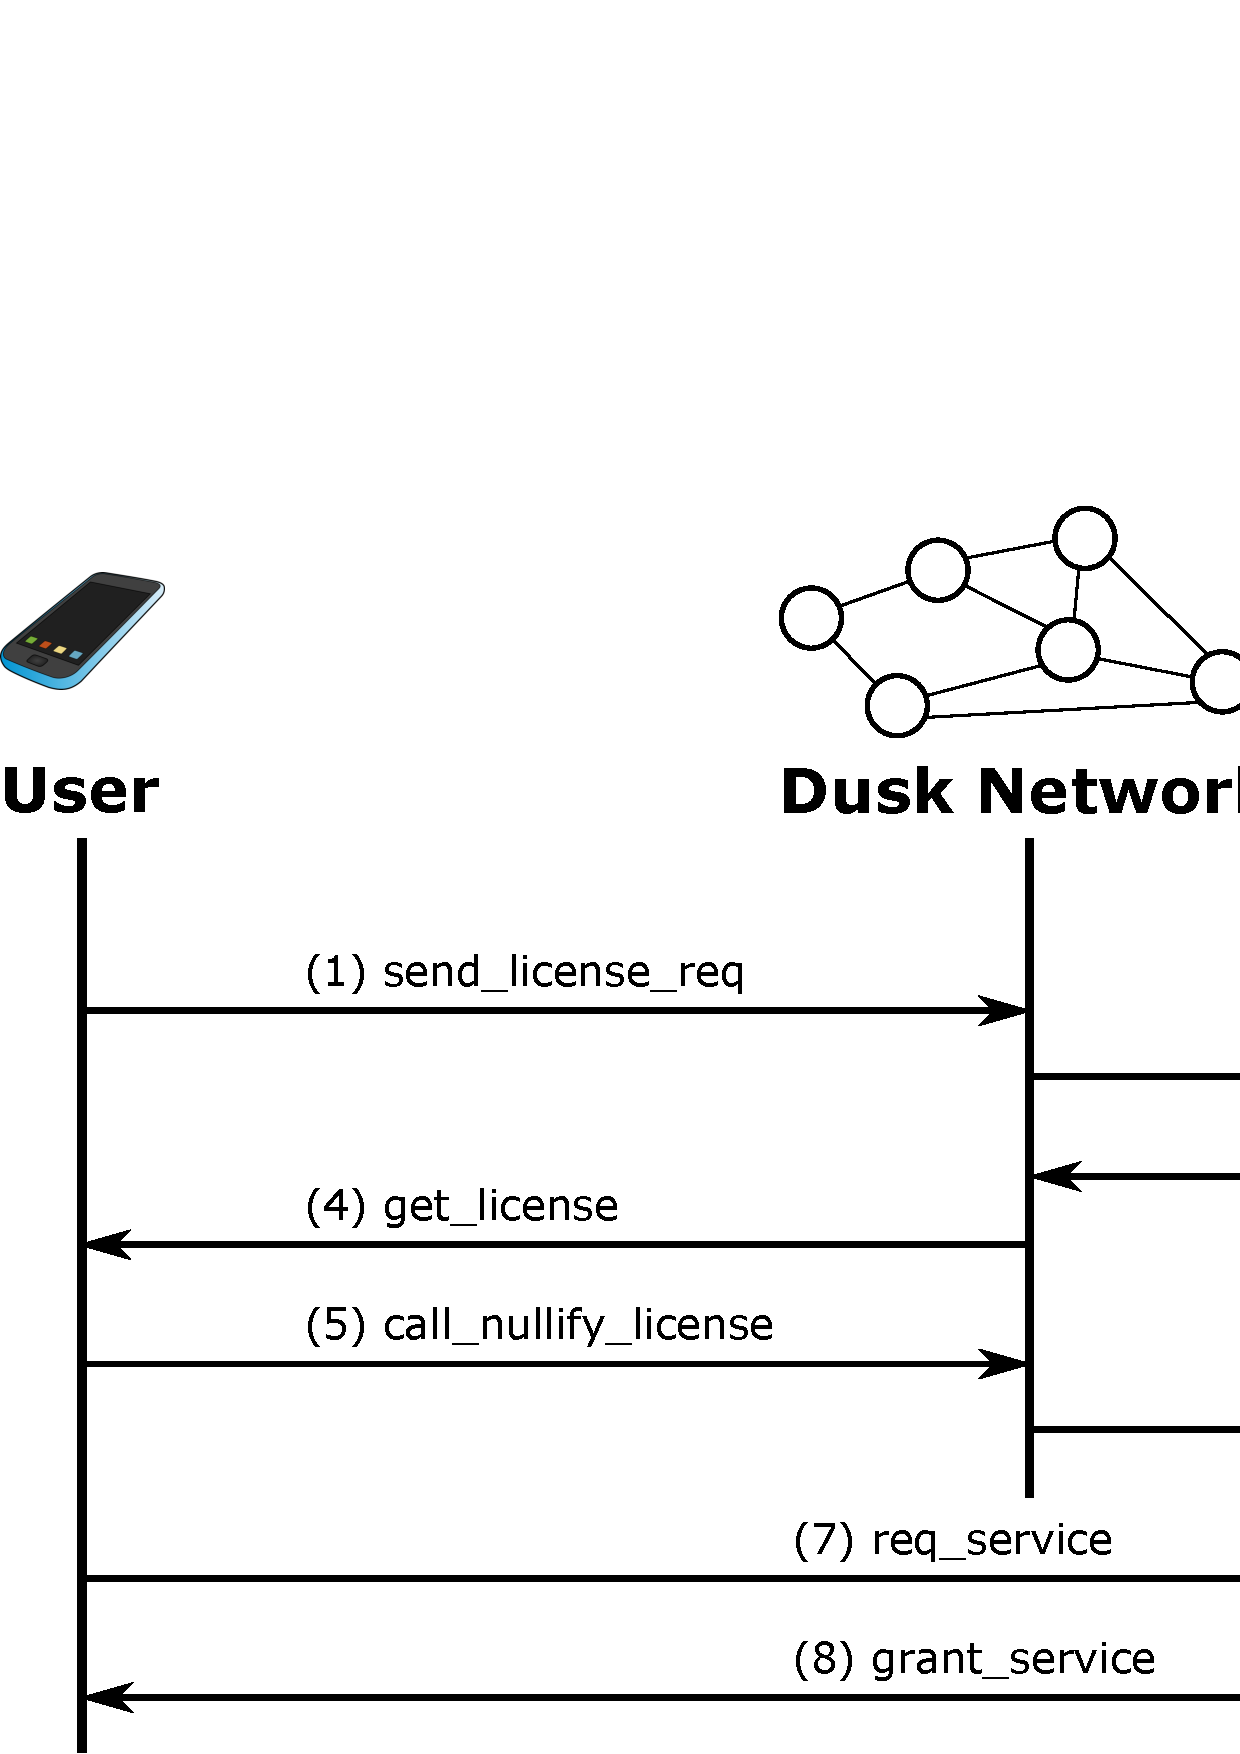
\includegraphics[width=.4\textwidth]{\figs/protocol.png}
	\caption{Overview of the protocol messages exchanged between the user, Dusk's network, and the LP/SP.}
	\label{fig:protocol}
\end{figure}



\section{Cryptographic primitives}
\label{sec:crypto-primitives}
% !TeX root = ../build/main.tex

{\color{red}{[TODO]}}

\subsection{Elliptic curves}

\mbi{Include details of Jubjub group, generators, etc.}

\subsection{Digital signatures}

\subsection{Encryption}

\subsection{Commitments}

\subsection{Proof systems}

\subsection{Hash functions}

\mbi{Hashing - it is going to be Poseidon everywhere.}

\subsection{Merkle trees}

\section{Protocol}
\label{sec:protocol}

The workflow is depicted in Figure \ref{fig:protocol}, and described with full details as follows.

\begin{figure}[h]
	\centering
		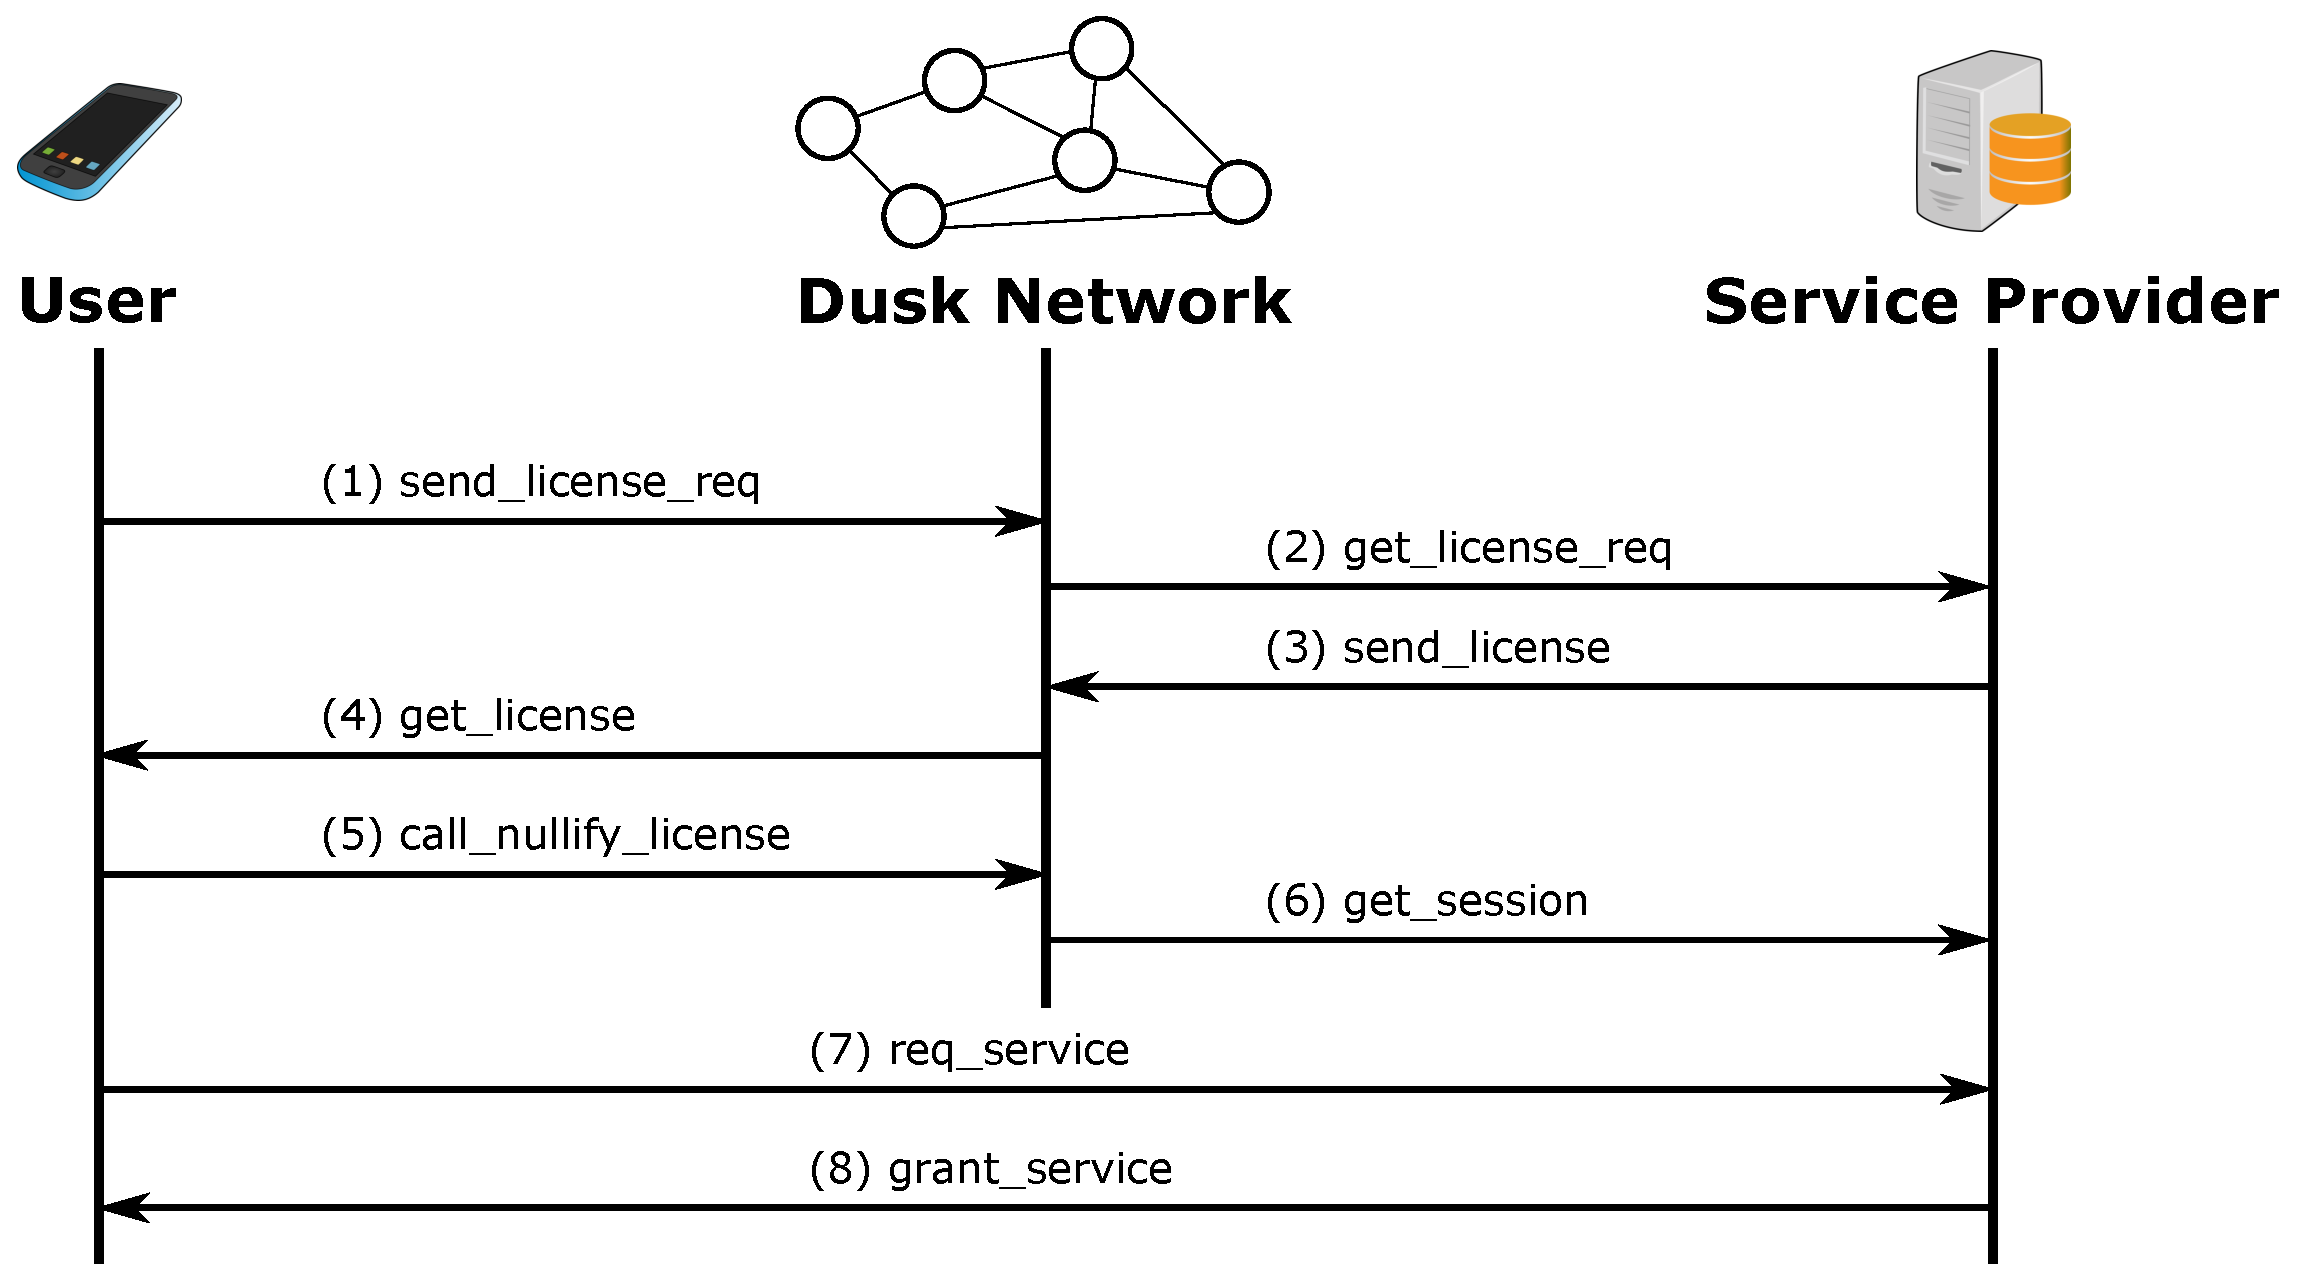
\includegraphics[width=390pt,draft=false]{images/protocol.eps}
	\caption{Overview of the protocol messages exchanged between the user, the Dusk Network, and the SP.}
	\label{fig:protocol}
\end{figure}

\begin{enumerate}
	\item (\textbf{user}) $\mathsf{send\_note\_license\_req}$ : Compute a note public key $(\npk_{\user}, R_{\user})$ belonging to the user, using the user's own public key, and also an additional key $\ksym_{\user} = \hp(\npk_{\user}, \nsk_{\user})$, by computing first the user's $\nsk_{\user}$. Then, send the required amount of Dusk coins to the SP, in order to pay for the service. Into the same transaction, send an NFT to the SP using the function $\mintnft(\npk_{\SP}, R_{\SP}, \nftpayload, \kdh)$, whose arguments are computed as follows:
	\begin{itemize}
		\item $(\npk_{\SP}, R_{\SP})$ is the SP's note public key, computed through his public key $\pk_{\SP}$.
		\item $\nftpayload = (\npk_{\user}, R_{\user}, \ksym_{\user})$.
		\item $\kdh$ is computed using the SP's public key.
	\end{itemize}

	\item (\textbf{SP}) $\mathsf{get\_note\_license\_req}$ : Continuously check the network for incoming license requests. Upon receiving the payment from a user, define a set of attributes $attr$ representing the license, and compute a digital signature as follows:

	$$\lsig= \sign_{\sk_{\SP}}(\npk_{\user}, \attr)$$

	\item (\textbf{SP}) $\mathsf{send\_note\_license}$ : Set the $\nftpayload = \{\lsig, \attr\}$, and send the license to the user using the function $\mintnft(\npk_{\user}, R_{\user}, \nftpayload, \ksym_{\user})$.

	\item (\textbf{user}) $\mathsf{get\_note\_license}$ : Receive the note containing the license. 

	\item (\textbf{user}) $\mathsf{call\_nullify\_license}$ : When desiring to use the license, nullify it by executing a call to the license contract. The following steps are performed:

	\begin{itemize}
		\item The user sets a session cookie $\stoken = (\mathsf{s_0}, \mathsf{s_1}, \mathsf{s_2}) \leftarrow \F_t$.
		\item The user creates a new NFT note where $\nftpayload = \stoken$, and the SP is the receiver.
		\item The user issues the transaction that includes the NFT described in the previous step, by calling the license contract. In this case, the \textsf{tx\_proof} is computed as done in the standard Phoenix model, but into the same circuit, the circuit depicted in Figure \ref{fig:circuit_prove_nft} is appended.
		\item The network validators will execute the smart contract, which verifies the proof. Upon success, the NFT note will be forwarded, and the license nullifier $\lnullifier$ will be added to the Merkle tree of nullifiers.
	\end{itemize}

	\item (\textbf{SP}) $\mathsf{get\_note\_session\_cookie}$ : Receive a note containing the session cookie $\stoken$.

	\item (\textbf{user}) $\mathsf{req\_service}$ : Request the service to the SP, establishing communication using a secure channel, and providing the tuple $(\mathsf{tx\_hash}, \pk_{\SP}, \attr, c, \stoken)$.

	\item (\textbf{SP}) $\mathsf{grant\_service}$ : Grant or deny the service upon verification of the following steps:

	\begin{itemize}
		\item Check whether or not the values $(\attr, \pk_{\SP}, c)$ are correct.
		\item Check whether or not the openings $((\pk_{\SP}, \mathsf{s_0}), (\attr, \mathsf{s_1}), (c, \mathsf{s_2}))$ match the commitments $\com_0^{hash}, \com_1, \com_2$ found in the transaction $\mathsf{tx\_hash}$.
	\end{itemize}

\end{enumerate}

\begin{figure}[h]
	\centering
	\setlength{\fboxsep}{5pt}%
	\setlength{\fboxrule}{0.3pt}%
	\fbox{
		
\includegraphics[width=460pt,draft=false]{images/circuit_prove_nft.eps}}
	\caption{Arithmetic circuit for proving a license's ownership.}
	\label{fig:circuit_prove_nft}
\end{figure}

Furthermore, the SP might request the user to nullify the license they are using (i.e. this is a single-use license, like entering a concert). This is done through the computation of $\lnullifier$. The deployment of this part of the circuit has two different possibilities:
\begin{itemize}
	\item If we set $c = 0$ (or directly remove this input from the circuit), the license will be able to be used only once.
	\item If the SP requests the user to set a custom value for $c$ (e.g. the date of an event), the license will be able to be reused only under certain conditions.
\end{itemize}


\section{Implementation details}
\label{sec:implementation}
% !TeX root = ../build/main.tex

\mbi{Add Milosz figure here or in {3. Protocol}?}

%\section{Abstract protocol}
%\label{sec:protocol-abstract}
%\input{\secs/protocol-abstract}
%
%\section{Concrete protocol}
%\label{sec:protocol-concrete}
%\input{\secs/protocol-concrete}

\bibliographystyle{splncs04.bst}
\bibliography{biblio.bib}

\end{document}
